\subsection{Generating the resource graph}
\label{sec:gener-reso-graph}

The resource graph represents the cluster of compute nodes on which
the task graph will be executed. A sample resource graph is shown in
fig \ref{fig:res} at level 0. The resource graph that is shown is truly
hetrogeneous in both computations and communication. The resource
graph is described below:

\begin{itemize}

\item The compute nodes are assumed to belong under two categories of
processing units, mainly CPUs and GPUs. The scalar instructions of a
Processing Element (\textbf{PE}) that represents a CPU is much higher
that that of a GPU. At the same time parallel vector operations that a
\textbf{PE} representing a GPU is much higher compared to that of a
CPU. In Fig \ref{fig:res} $ R^1 $ is a 'CPU' and $ R^5 $ is a 'GPU'.

\item In the resource graph shown in Fig \ref{fig:res} at level 0, the
interconnect between these PEs are considered to be a two dimensional
mesh. In this topology the PEs are connected in a grid with individual
communication links between them. The bandwidth of these links are
considered to be non uniform. Similarly, it is possible to represent
various resource graphs with different topologies.

\end{itemize}

Mapping the task graph on to such a hetrogeneous is NP hard. The
problem mainly lies in the size of the resouce graph and the number of
ways in which the task graph can be mapped on to the resource graph.

In our approach we tackle the problem in several phases. The various
stages that are performed is shown here:

\begin{itemize}

\item Firstly, we form virtual representations of the resource graph by
clustering the nodes. These virtual nodes are formed by min cutting
communication volume and load balancing the virtual nodes capabilities.
The formation of these virtual nodes creates homogeneous partitions
from hetrogeneous PEs.

\item Secondly, instead of doing this in a single step, we construct
this in several level by clustering half the nodes from the previous
level. We end up with a structure consisting of several levels, where
the $ Number\ of\ levels = log_2 ( Number\ of\ Nodes )$.

\item The communication bandwidth between the clustered nodes is
determined by,\\ ${ \sum ( \min for same destn ( \max bw R^i, R^j ) )
) }$\\ The max bandiwdths between any ${R^i}$ is determined by floyd
warshall algorithm.

\item The capabity of each of the PEs that are clustered together are
aggregated to form the larger virtual node.

\item In each level PEs with high communication bandwidth and balanced
capabilities are clustered together. In doing this in a bottom up
approach i.e. clustering instead of partitioning, we allow the nodes to
form without ignoring communication links between the nodes. This also
avoids the formation of dangling nodes in the graph.

\end{itemize}

\begin{figure}[ht]
  % \centering
  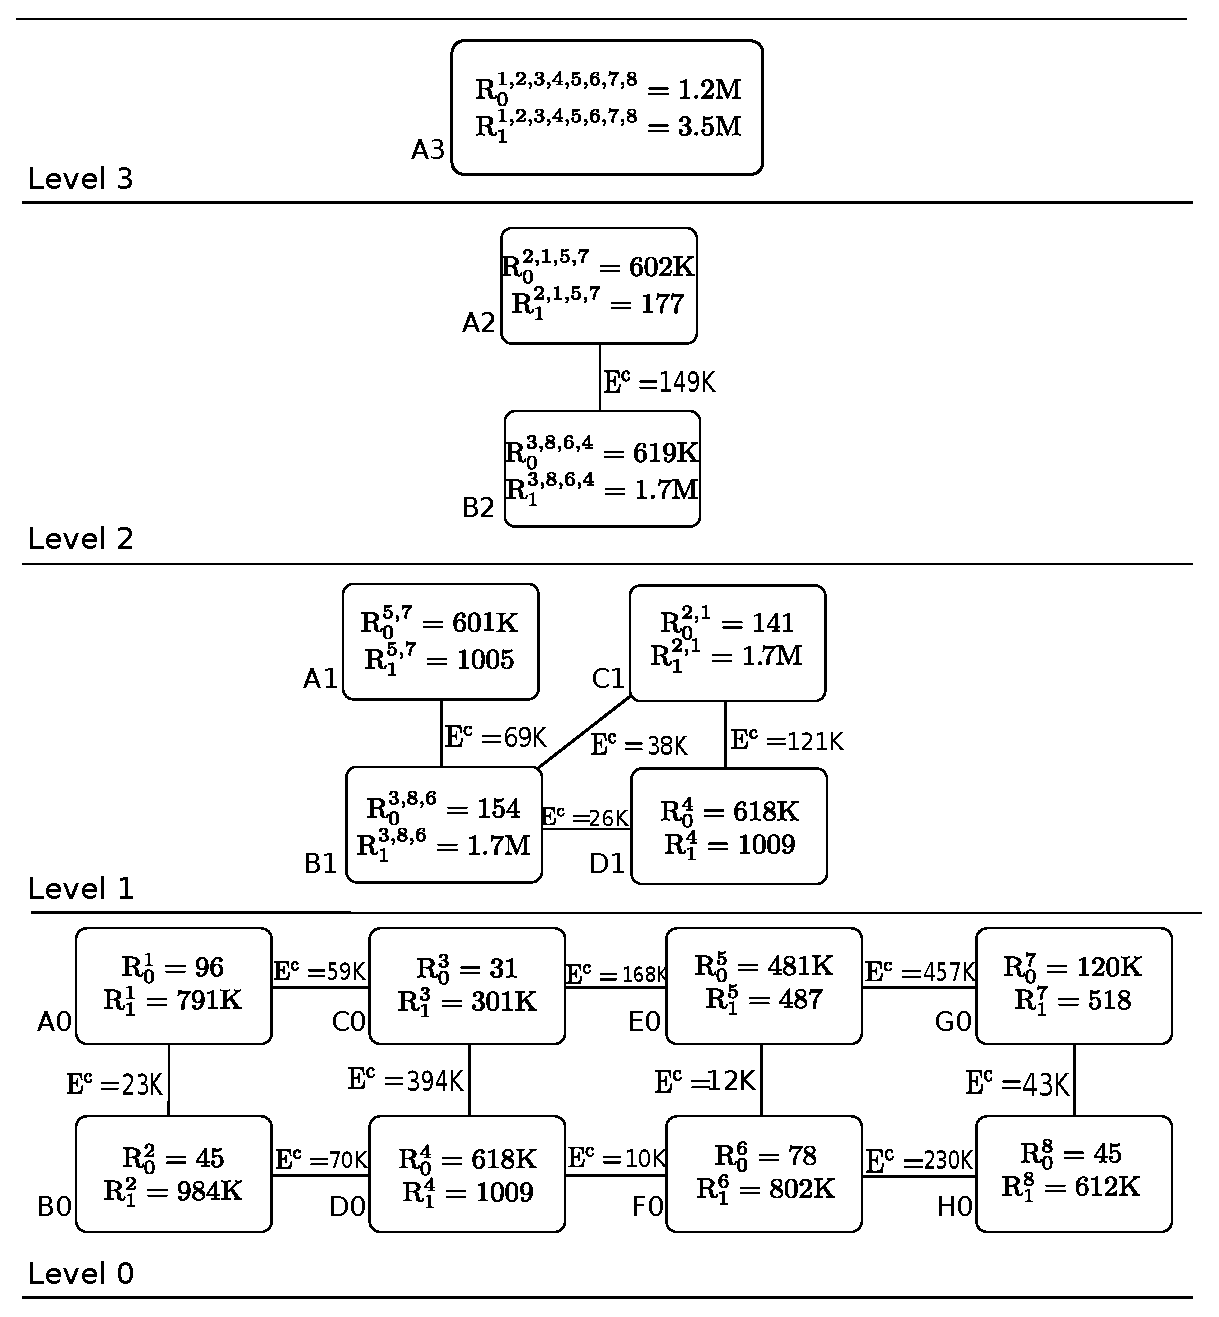
\includegraphics[scale=0.43]{./figures/resource}
  \caption{Clustering of a resource graph}
  \label{fig:res}
\end{figure}

In fig \ref{fig:res} we show our clustering approach on a 4x2 mesh. At
each level suitable nodes are clustered together to form a larger node.
We see that the PE $ R^3 $ and PE $ R^8 $ are combined together
when moving from level 0 to level 1. Overall, we reach three levels
and at the top most level all the nodes from a single virtual node.

\subsection{Application partitioning}
\label{sec:appl-part}




